\documentclass[14pt]{extarticle}

\usepackage{titlesec}
\usepackage{titling}
\usepackage{url}
\usepackage[margin=.5in]{geometry}
\usepackage{xcolor}
\usepackage{setspace}
\usepackage{listings}
\usepackage{graphicx}
\usepackage{ulem}
\usepackage{enumitem}
\usepackage{hyperref}

\title{FastAPI from a CRUDmaker's POV: A Start-to-Finish Example}
\author{Daniil Kraynov -- \href{https://parkanaur.net}{parkanaur.net}}

% Text/list formatting
\hypersetup{colorlinks=true, urlcolor=blue}
\onehalfspacing
\setlist{noitemsep}
\newcommand{\sectionbreak}{\clearpage}
\setcounter{tocdepth}{2}

% URL footnotes and note macro
\newcommand{\flink}[1]{\footnote{\href{#1}{#1}}}
\newcommand{\note}{\textbf{\color{red}Note: }}

% Generic code listing style - c means code, not C
\lstdefinestyle{cstyle}{
    numbers=left,
    basicstyle=\ttfamily\small,
    commentstyle=\color{darkgray}\small,
    keywordstyle=\color{blue}\bfseries,
    morekeywords={*,
    % bash
    poetry, git, mv, python,
    % Python
    async},
    showstringspaces=false,
    aboveskip=0.5cm,
    xleftmargin=0.5cm,
    framesep=0mm,
    frame=tb,
    framexleftmargin=0.75cm,
    columns=fullflexible,
    breaklines=true}

\lstnewenvironment{code}[1]{\lstset{
    language=#1,
    style=cstyle}}{}

% Inline code
\newcommand{\cinline}[2]{{\lstinline[language=#1, style=cstyle, basicstyle=\ttfamily\normalsize]{#2}}}

\begin{document}

\maketitle

% TOC
{\hypersetup{linkcolor=black}
\tableofcontents}

\section{Introduction}

FastAPI, a high-performant Python web framework, is very well documented, but the documentation might be a bit too overwhelming for a semi-seasoned developer who already has experience with designing web applications and has a general stance on how they should be structured.

I've started writing this article as a compilation of notes to refer to when writing an app in FastAPI from the ground up. The end result of my initial tinkering with FastAPI, documented here, is a file hosting application with a bunch of extras like Docker integration.

Due to FastAPI being an ASGI framework, deployment process is a little bit different from using nginx and uWSGI, so I hope to cover the deployment caveats as well.

\subsection{Who is this article intended for}

This article aims to help developers coming from other frameworks (Flask, Django, as well as non-Python ones) who know what they're doing and are willing to jump straight into action but don't feel like getting overwhelmed with deeper aspects of FastAPI's official documentation \flink{https://fastapi.tiangolo.com} (I still advise everyone to read it - it's good on its own and is quite helpful!).

It could also be of good use to beginner developers, but some aspects of this article \textit{might} be harder to understand for them - please give feedback on whether it's a good read or not!

\subsection{Application structure}

From my experience, the general workflow for producing a mid-sized web application is as follows:

\begin{enumerate}
    \item Designing a set of domain model classes (e.g. User, Item, etc.)
        \begin{enumerate}
            \item Choosing a data source
            \item Likely some automatic migration scripts
        \end{enumerate}
    \item Creating an API skeleton for at least one entity
        \begin{enumerate}
            \item Authentication logic
        \end{enumerate}
    \item Adding a business logic layer for at least one entity
    \item Binding it all together
    \item Adding logic/API for the rest of the entities
    \item {[optional]} Adding a frontend and a bunch of non-logic pages (in parallel with the previous steps or after them, depending on size of the developing team)
    \item {[semi-optional]} Deploy scripts, tests, CI/CD, etc.
\end{enumerate}

FastAPI's documentation describes or mentions most of these steps, but in no specific order. For an experienced developer there are pages of particular interest (e.g. app structure for bigger applications \flink{https://fastapi.tiangolo.com/tutorial/bigger-applications/}, but from there you have to go deeper into the documentation in order to find out how to structure your models, DTOs, etc.

You'd probably start jumping around more and more around the documentation, get overwhelmed with the amount of points (most likely you wouldn't need all of them at the start of your FastAPI journey), and, in the worst case, lose motivation in learning FastAPI - it happened to me at first, which is a shame, because FastAPI is a beautiful framework!

\subsection{Feedback}

I don't consider myself an expert in either programming, documentation, or English, and this article is certain to have bad architecture decisions or mishaps in general.

I encourage you to send your comments regarding this article, whether they're about me doing a good job or being an ignorant fool who doesn't know any better (I'm serious on this one!). Maybe you can think of a few additions as well, in which case you can also fork this article - it's "licensed" under CC0, so you're free to do whatever you want with it.

You can send your comments via GitHub issues/PRs \flink{https://github.com/parkanaur/fastapi-notes} or by sending an e-mail at {\href{mailto:dan@parkanaur.net}{dan @ parkanaur.net}}. Don't hesitate!

\section{Preparations}

The project that I'm going to describe is \textbf{PyFH} \flink{https://github.com/parkanaur/pyfh}, a file hosting application designed for self-hosting, with a few additional features like public/private files, timed files, encryption, etc.

I'll try to follow the incremental model, starting at the very basic things like setting up environment all the way to deployment on a real world VPS.

\subsection{Setting up environment}

It seems that the good old requirements.txt is slowly falling out of favor within the Python ecosphere, so we're gonna \sout{bite the bullet} follow suit and use the newer toolset (i.e. Poetry). This is a good exercise in using non-standard tooling as well.

Poetry is supposed to make managing virtualenvs and dependencies easier, so let's go ahead and install it \flink{https://python-poetry.org/docs/}.

You can use regular requirements.txt instead - be sure to remove Poetry-related lines and replace them with manual venv creation (\cinline{bash}{python -m venv venv}).

\begin{code}{bash}
    # Poetry will create the project directory for you automatically
    cd ~/code
    poetry new pyfh
    cd pyfh
    git init

    # Virtualenv creation/activation (deactivate with exit)
    poetry shell

    # Don't @ me
    mv README.rst README.md
\end{code}

Time to add a few dependencies. We're building a file hosting app, so we're gonna need a few extras for our FastAPI dependency. It's a good idea to just add the whole \texttt{fastapi[all]} dependency during development - it adds multipart support, as well as a few more goodies, and if you care about the amount of your dependencies, you can clean the unneeded stuff out later.

\texttt{fastapi[all]} also installs \texttt{uvicorn[standard]} as per FastAPI installation tutorial.

\note Most of the bash commands will imply that you have activated your virtualenv (\cinline{bash}{poetry shell}).

\begin{code}{bash}
    # Install our dependency - same as (pip install + freeze > requirements.txt)
    # If you're using zsh, enclose fastapi[all] in quotes
    poetry add fastapi[all]
\end{code}

Now we're ready to start adding more stuff into the project.

\subsection{Initial project structure}

First we have to add some boring stuff - a few folders with empty \texttt{\_\_init.py\_\_}'s in them, a barebones main.py file, .gitignore, etc.

\subsubsection{gitignore}

Github's Python gitignore will do just fine \flink{https://github.com/github/gitignore/blob/master/Python.gitignore}.

\note You don't need to add \texttt{poetry.lock} to .gitignore - it's used to freeze currently installed (on your machine) package versions (similar to versions in \texttt{requirements.txt}). Poetry will make use of that file in other developers' machines to produce the same environment as you. You can later run \cinline{bash}{poetry update} to use newer package versions.

\subsubsection{main.py}

This is similar to \texttt{main.py/wsgi.py} in Flask - an ASGI server will use it as a starting point for your application (same as passing \texttt{main:app} to uWSGI, if you will).

Let's add the simplest \cinline{bash}{main.py} possible for now:

\begin{code}{Python}
    from fastapi import FastAPI

    app = FastAPI()

    @app.get("/")
    async def test():
    return "Welcome to pyfh!"
\end{code}

Let's try it out. Uvicorn is used to launch ASGI apps \flink{https://www.uvicorn.org/deployment/} (we'll cover production deployment later), --reload enables auto-restart on code changes:

\begin{code}{bash}
    uvicorn main:app --reload
    # ..... ^^^^---- main.py
    # ..... -----^^^ app = FastAPI()
\end{code}

Alternatively you can call \cinline{Python}{uvicorn.run()} in main.py, rather than use the command-line tool.

Then make an HTTP request to 127.0.0.1:8000 and you should see something along the lines of the following:

\begin{figure}[h]
    \centering
    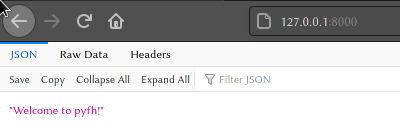
\includegraphics[width=0.7\textwidth]{img/helloworld.png}
    \caption{Hello World in FastAPI}
\end{figure}

\subsubsection{Folders and \texttt{\_\_init.py\_\_'s}}

Time to add some more structure. Files not in the root directory \textbf{are empty} unless otherwise noted.

{\ttfamily
\begin{itemize}
    \item{$\sim$/code/pyfh}
        \begin{itemize}
            \item{main.py}
            \item{pyproject.toml}
            \item{poetry.lock}
            \item{.gitignore}
            \item{README.md}
            \item{Dockerfile *}
            \item{.dockerignore *}
            \item{docker-compose.yaml *}
            \item{pyfh/}
                \begin{itemize}
                    \item{\_\_init.py\_\_}
                    \item{entities/}
                        \begin{itemize}
                            \item{\_\_init.py\_\_}
                            \item{user.py}
                        \end{itemize}
                    \item{routes/}
                        \begin{itemize}
                            \item{\_\_init.py\_\_}
                            \item{user.py}
                        \end{itemize}
                \end{itemize}
        \end{itemize}
\end{itemize}
}

You may have noticed the presence of Docker-related files. We'll get to writing them later on. As much as I hate to admit it, Docker's just too useful sometimes.

\section{Domain Model and Data Source}

\subsection{Creating entities}

\end{document}
